\subsection{Цель выполнения домашнего задания}\label{blockN.VariantM}
\textbf{Цель выполнения домашнего задания }-- \GoalOfResearch

%-------------------------------------------------
\subsection{Задание}
Система состоит из устройств типа $A$ и типа $B$, интенсивности отказов $\lambda_A$ и $\lambda_B$ известны.
Для функционирования системы требуется хотя бы одно устройство типа $A$ и хотя бы $N_B$ устройств типа $B$.
Общее число устройств в системе (включая резервные) – $R_A$ и $R_B$ соответственно,
причём в нормальном состоянии одновременно включены сразу $N_A$ устройств типа $A$.

Если $N$ – номер зачётной книжки, а $G$ – последняя цифра в номере группы,
то параметры системы определяются следующим образом:
\[
\begin{matrix}
    \lambda_A= G + (N \bmod 3) \\
    \lambda_B= G + (N \bmod 5) \\
    N_A= 2 + (G \bmod 2) \\
    N_B= 2 + (N \bmod 2) \\
    R_A= 4 + (G \bmod 2) \\
    R_B= 5 - (G \bmod 2)
\end{matrix}
\]

Требуется:
\begin{enumerate}
    \item нарисовать граф состояний системы;
    \item составить матрицу интенсивностей переходов;
    \item записать дифференциальные уравнения Колмогорова;
    \item аналитически решить полученную систему уравнений, исходя из того, что в начальный момент времени все устройства исправны;
    \item построить графики вероятностей нахождения системы в каждом из возможных состояний с течением времени;
    \item построить график функции надёжности системы;
    \item рассчитать математическое ожидание времени безотказной работы;
    \item провести имитационное моделирование системы в терминах непрерывных марковских цепей 100 раз, рассчитать среднее выборочное значение и стандартное отклонение времени безотказной работы системы.
\end{enumerate}
%-------------------------------------------------
\newpage
\subsection{Решение}

Рассчитаем начальные данные для выполнения домашнего задания по номеру зачетки $N = {{ var }}$ и группы $G = {{ g }}$:
\[
\begin{matrix}
    \lambda_A & = G + (N \bmod 3) = {{ g }} + ({{ var }} \bmod 3) = & {{ g + var % 3}} \\
    \lambda_B & = G + (N \bmod 5) = {{ g }} + ({{ var }} \bmod 5) = & {{ g + var % 5}} \\
    N_A & = 2 + (G \bmod 2) = 2 + ({{ g }} \bmod 2) = & {{ 2 + g % 2 }} \\
    N_B & = 2 + (N \bmod 2) = 2 + ({{ var }} \bmod 2) = & {{ 2 + var % 2 }} \\
    R_A & = 4 + (G \bmod 2) = 4 + ({{ g }} \bmod 2) = & {{ 4 + g % 2 }} \\
    R_B & = 5 - (G \bmod 2) = 5 - ({{ g }} \bmod 2) = & {{ 5 - g % 2 }}
\end{matrix}
\]
Предположим что $S^{ab}_{cd}$ - состояние системы, где
\begin{itemize}
    \item $a$ - количество работающих устройств типа $A$, включая резервные,
    \item $b$ - количество резервных устройств типа $A$,
    \item $c$ - количество работающих устройств типа $B$, включая резервные,
    \item $d$ - количество резервных устройств типа $B$.
\end{itemize}
На рисунке \ref{graph} изображен граф состояний системы.


\begin{figure}[H]
\centerline{ {{ G }} }
\caption{Граф состояний системы}
\label{graph}
\end{figure}

\newpage
Переобозначим состояния следующим образом: {{ renumerate }}.

На основании построенного графа состояний можно составить матрицу интенсивностей переходов (матрица \ref{matrix}).
Необходимо заметить, что диоганальные элементы матрицы равны отрицательной сумме всех остальных элементов строки.

\[
    \resizebox{\textwidth}{!}{$
    \Lambda =
    \begin{pmatrix}
    {{ mat }}
    \end{pmatrix}
    \tag{1} \label{matrix}
    $}
\]

\newpage

Составим систему дифференциальных уравнений Kолмогорова.
\[
\begin{cases}
    {{ kolmogorov }}
\end{cases}
\]

Начальные условия:
$$P_0(t=0)=1$$
$$P_i(t=0)=0 \quad \forall i \in [1, {{ pathsN }}]$$

Найдем функцию $P_0(t)$.
\begin{gather*}
    \frac{dP_0(t)}{dt} = -{{ Na * lambda_A + Nb * lambda_B }} P_0 (t)\\
    \int \frac{1}{P_0 (t)} d P_0(t) = \int -{{ Na * lambda_A + Nb * lambda_B }} dt\\
    \int d \ln P_0 (t) = \int -{{ Na * lambda_A + Nb * lambda_B }} dt\\
    \ln P_0 (t) = -{{ Na * lambda_A + Nb * lambda_B }} t + c\\
    P_0 (t) = e^{-{{ Na * lambda_A + Nb * lambda_B }} t + c}\\
    P_0(t = 0) = 1 => e^{-{{ Na * lambda_A + Nb * lambda_B }} t + c} = 1 => c = 0\\
    P_0 (t) = e^{-{{ Na * lambda_A + Nb * lambda_B }} t}\\
\end{gather*}

Теперь найдем функцию $P_1 (t)$
\begin{gather*}
    \frac{d P_1(t)}{dt} = {{ Nb * lambda_B }} e^{-{{ Na * lambda_A + Nb * lambda_B }} t} - {{ Na * lambda_A + Nb * lambda_B }} P_1(t)\\
    \frac{d P_1(t)}{dt} + {{ Na * lambda_A + Nb * lambda_B }} P_1(t) = {{ Nb * lambda_B }} e^{ -{{ Na * lambda_A + Nb * lambda_B }} t} \quad |\cdot e^{ {{ Na * lambda_A + Nb * lambda_B }} t} \\
    e^{ {{ Na * lambda_A + Nb * lambda_B }} t} \frac{d P_1(t)}{dt} + e^{ {{ Na * lambda_A + Nb * lambda_B }} t} {{ Na * lambda_A + Nb * lambda_B }} P_1(t) = {{ Nb * lambda_B }}\\
    \frac{d P_1(t) \cdot e^{ {{ Na * lambda_A + Nb * lambda_B }} t }}{dt} = {{ Nb * lambda_B }}\\
    \int \frac{d P_1(t) \cdot e^{ {{ Na * lambda_A + Nb * lambda_B }} t } }{dt} dt = \int {{ Nb * lambda_B }} dt\\
    P_1(t) e^{ {{ Na * lambda_A + Nb * lambda_B }} t } = {{ Nb * lambda_B }} t + c => P_1(t) = ( {{ Nb * lambda_B }} t + c) e^{ -{{ Na * lambda_A + Nb * lambda_B }} t } \\
    P_1(t=0) = 0 => ( 0 + c ) e^{ -{{ Na * lambda_A + Nb * lambda_B }} t } = 0 => c=0\\
    P_1(t) = {{ Nb * lambda_B }} e^{ -{{ Na * lambda_A + Nb * lambda_B }} t } t\\
\end{gather*}

Аналогично вычисляется $P_2 (t)$:
\begin{gather*}
    P_2(t) = {{ Na * lambda_A }} e^{- {{ Na * lambda_A + Nb * lambda_B }} t}t\\
\end{gather*}

На основе $P_1 (t)$ и $P_2 (t)$ найдем $P_4 (t)$:
\begin{gather*}
    \frac{d P_4(t)}{dt} = {{ Nb * lambda_B }} P_1 (t) + {{ Na * lambda_A }} P_2 (t) - {{ Na * lambda_A + Nb * lambda_B }} P_4(t)\\
    \frac{d P_4(t)}{dt} + {{ Na * lambda_A + Nb * lambda_B }} P_4(t) = {{ (Na * lambda_A * Nb * lambda_B) * 2 }} e^{- {{ Na * lambda_A + Nb * lambda_B }} t} t\\
    \frac{d}{dt} (e^{ {{ Na * lambda_A + Nb * lambda_B }} t} P_4(t)) = {{ (Na * lambda_A * Nb * lambda_B) * 2 }} t\\
    \int \frac{d}{dt} (e^{ {{ Na * lambda_A + Nb * lambda_B }} t} P_4(t)) dt = \int {{ (Na * lambda_A * Nb * lambda_B) * 2 }} t dt\\
    e^{ {{ Na * lambda_A + Nb * lambda_B }} t} P_4(t) = {{ Na * lambda_A * Nb * lambda_B }} t^2 + c \\
    y(0) = 0 => P_4(t) = e^{ -{{ Na * lambda_A + Nb * lambda_B }} t} ( {{ Na * lambda_A * Nb * lambda_B }} t^2 + c), c = 0 \\
    P_4(t) = {{ Na * lambda_A * Nb * lambda_B }} e^{ -{{ Na * lambda_A + Nb * lambda_B }} t} t^2\\
\end{gather*}

\newpage
По аналогии с $P_1 (t)$, $P_2 (t)$ и $P_4 (t)$ вычислим функции вероятностей для всех нетерминальных состояний:
\begin{gather*}
    {{ P_funcs }}
\end{gather*}

По вычисленным функциям были построены графики вероятностей нахождения системы в каждом из возможных <<рабочих>> состояний с течением времени (рис. \ref{P_0} и \ref{P_i}).
\begin{figure}[H]
\centerline{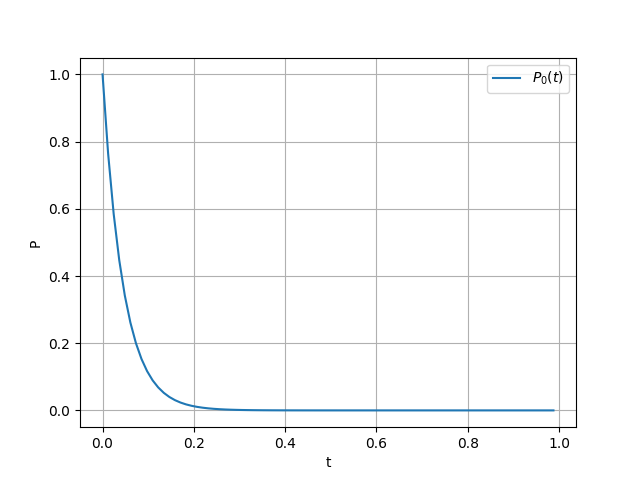
\includegraphics[scale = 0.8]{Images/graph_0.png}}
\caption{Функция вероятности для начального состояния}
\label{P_0}
\end{figure}

\begin{figure}[H]
\centerline{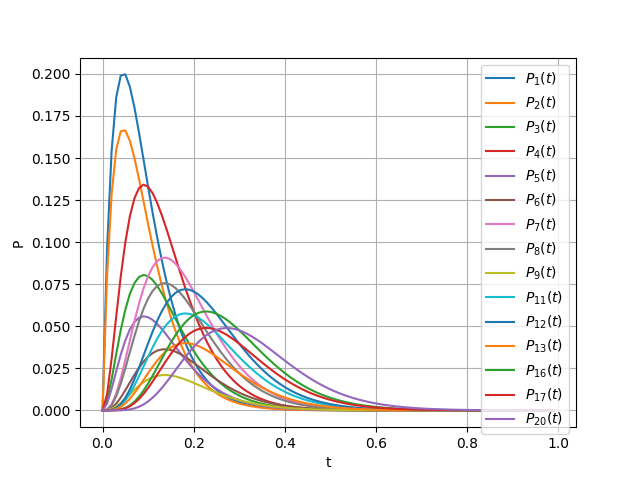
\includegraphics[scale = 0.8]{Images/graph.png}}
\caption{Функции вероятностей для нетерминальных состояний}
\label{P_i}
\end{figure}

Найдем функцию вероятности системы для терминального состояния.

\begin{align*}
    P_{term}&=1 - \sum P_{not\_term}
\end{align*}
\begin{equation}
    \begin{aligned}
    P_{term} = 1 - e^{-{{ Na * lambda_A + Nb * lambda_B }} t} ( {{ P_term }} )
    \end{aligned}
\end{equation}

График функции вероятности терминального состояния представлен на рисунке \ref{Term_t}.

\begin{figure}[H]
\centerline{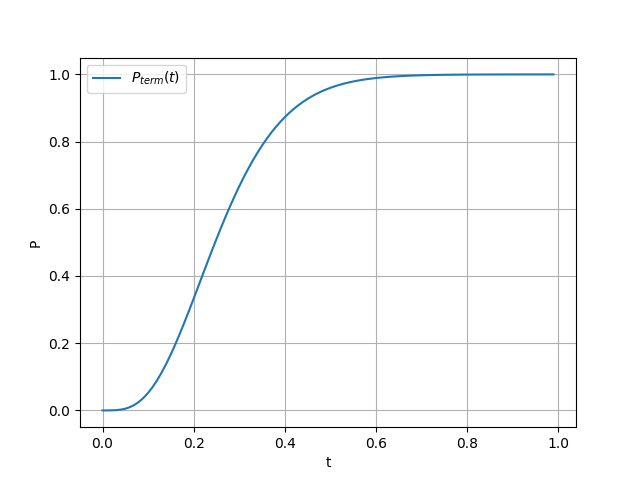
\includegraphics[scale = .8]{Images/Term_t.png}}
\caption{График функции вероятности терминального состояния}
\label{Term_t}
\end{figure}

\subsubsection{Функция надежности системы}

Функция надежности может быть определена следующим образом:
$$R(t)= 1 - P_{term}(t)$$

График функции надежности $R(t)$ представлен на рисунке \ref{R_t}.
\begin{figure}[H]
\centerline{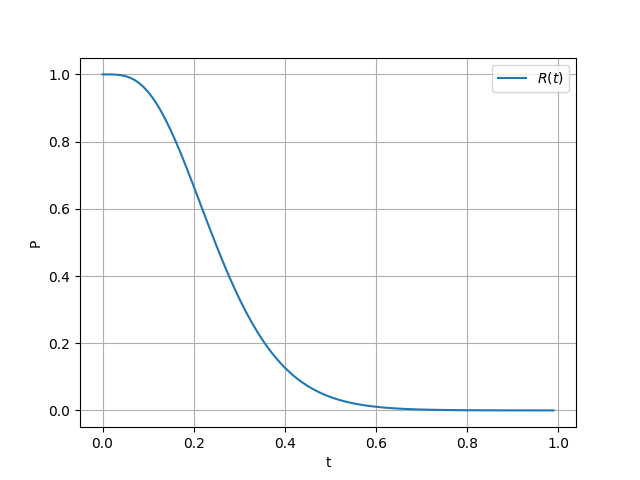
\includegraphics[scale = .8]{Images/R_t.png}}
\caption{Функция надежности системы}
\label{R_t}
\end{figure}
Математическое ожидание может быть вычислено по следующей формуле:
$$\mu = \int\limits_0^{+\infty}R(t)dt = {{ mu }}$$

\subsubsection{Имитационное моделирование}

Для системы с непрерывным временем была реализована функция, осуществляющая переходы по состояниям.

\begin{lstlisting}[language=python, label=prog,caption={\textit{реализация марковского процесса}}]
# моделирование одного эпизода с непрерывным временем
def MD(m):

    def F_t(l,y):
        return -np.log(1-y)/l


    def find_lambda(line):
        flag = True
        for i in range(len(line)):
            if line[i] > 0:
                if flag:
                    lb = [i, line[i]]
                    flag = False
                else:
                    la = [i, line[i]]

        return lb, la

    current_s = 0
    current_t = 0
    states_tr = [current_s]
    t_tr = [0]

    while np.max(m[current_s]) != 0:  # пока не упали в терминальное
        lb, la = find_lambda(m[current_s])
        t_cur_s=F_t(la+lb, np.random.uniform(low=0.0, high=1.0, size=None))  # -log(1-y)/(lambda_a+lambda_b)

        current_t += t_cur_s
        idx_b=m[current_s].index(lb)
        idx_a=list(m[current_s])[idx_b+1::].index(la) + idx_b + 1
        current_s = np.random.choice([idx_a, idx_b], p=[la/(la+lb), lb/(la+lb)])

        # для дальнейшей отрисовки
        states_tr.append(current_s)
        t_tr.append(current_t)

    return current_t, states_tr, t_tr
\end{lstlisting}

На рисунке \ref{MDP} представлен график переключению состояний системы для 15 прогонов ($N=15$).
\begin{figure}[H]
\centerline{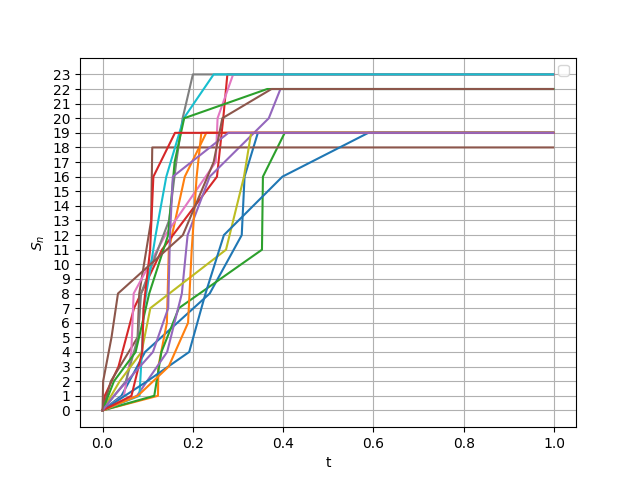
\includegraphics[scale = .8]{Images/term.png}}
\caption{График переключению состояний системы}
\label{MDP}
\end{figure}

Для $N=100$
$$S=\sqrt{D\frac{N}{N-1}}= {{ sred_o }},$$
$$\hat{t}={{ st_o }},$$
где $S$ - стандартное, $\hat{t}$ - среднее отклонение.

%-------------------------------------------------
\subsection{Вывод}
В ходе выполнения домашнего задания была промоделирована работа СМО в терминах непрерывных марковских цепей,
а также выполнен анализ ее работы.

% --------------------------------------
% Атрибуты задачи
\labattributes{}{}{}{}{студент группы \EduGroup, \Author}{\Year, \Semestr}
%--------------

